\chapter{Introduction}
\onehalfspacing

\section{Background and Motivation}

Every minute, hundreds of hours of video content are uploaded to platforms like YouTube, Instagram, and ShareChat --- and a growing fraction of that content comes from Indian creators who express themselves in a fluid blend of Hindi and English. These creators are not code-switching as an afterthought; they are speaking naturally, as millions of urban Indians do every single day. Yet when a sentiment analysis system processes their words, it almost always fails. The models were not built for them.

Sentiment analysis (SA) is the computational task of automatically determining the emotional polarity of a piece of content --- whether the speaker or author is expressing something positive, negative, or neutral \cite{liu2012sentiment}. Since its early roots in opinion mining and product review classification, the field has matured considerably. It now underpins brand monitoring dashboards, mental health screening tools, financial market prediction systems, and political discourse analytics \cite{wankhade2022survey}. The economic incentive alone is enormous: companies routinely spend millions of dollars trying to understand what their customers actually feel, and automated sentiment analysis is a scalable answer to that question \cite{cambria2016affective}.

For most of its history, however, sentiment analysis has operated on a single input channel --- typically written text. This is a significant simplification. Human communication is inherently multimodal: we express ourselves through the words we choose, the way we say them, and the expressions on our faces. A sentence like ``Oh, absolutely brilliant'' means something completely different when spoken slowly with a raised eyebrow than when delivered with a genuine smile. Any system that processes only the words, ignoring the acoustic and visual channels, will routinely misread sarcasm, irony, and emotional nuance \cite{poria2017review}.

\textit{Multimodal Sentiment Analysis} (MSA) addresses this gap by jointly modelling text, audio, and visual signals. The field gained significant momentum with the introduction of the CMU-MOSI dataset \cite{zadeh2016mosi}, which provided aligned transcripts, audio features, and video frames for thousands of English opinion segments. Subsequent work extended this to larger corpora (CMU-MOSEI \cite{zadeh2018multimodal}) and more controlled emotional settings (IEMOCAP \cite{busso2008iemocap}), enabling the development of increasingly sophisticated fusion architectures \cite{tsai2019multimodal, hazarika2020misa, pham2019found, yang2021mtag}. Figure~\ref{fig:msa_overview} illustrates the general framework: three modality streams are independently encoded and then combined through a cross-modal fusion mechanism to produce a continuous sentiment score.

\begin{figure}[ht]
\centering
\begin{tikzpicture}[
    node distance=0.55cm and 1.3cm,
    box/.style={draw, rounded corners=3pt, minimum width=2.5cm, minimum height=0.62cm, align=center, font=\small},
    enc/.style={draw, rounded corners=3pt, fill=blue!10, minimum width=2.5cm, minimum height=0.68cm, align=center, font=\small},
    proj/.style={draw, rounded corners=3pt, fill=yellow!25, minimum width=2.5cm, minimum height=0.55cm, align=center, font=\scriptsize},
    fuse/.style={draw, rounded corners=5pt, fill=orange!15, minimum width=9.0cm, minimum height=0.85cm, align=center, font=\small\bfseries},
    sentout/.style={draw, rounded corners=5pt, fill=green!15, minimum width=4.5cm, minimum height=0.72cm, align=center, font=\small\bfseries},
    arr/.style={->, thick}
]
\node[box] (txt) {Text Transcript};
\node[box, right=of txt] (aud) {Audio Waveform};
\node[box, right=of aud] (vis) {Video Frames};

\node[enc, below=of txt]  (tenc) {MuRIL\\\scriptsize{768-dim}};
\node[enc, below=of aud]  (aenc) {wav2vec2-XLSR\\\scriptsize{1024-dim}};
\node[enc, below=of vis]  (venc) {CLIP ViT-B/32\\\scriptsize{512-dim}};

\node[proj, below=of tenc] (tp) {Linear Proj. (128-d)};
\node[proj, below=of aenc] (ap) {Linear Proj. (128-d)};
\node[proj, below=of venc] (vp) {Linear Proj. (128-d)};

\node[fuse, below=1.25cm of ap] (fus) {Cross-Modal Attention Fusion \ --- \ MulTHinglish};
\node[sentout, below=0.75cm of fus] (sentnode) {Sentiment Score $\in [-3,\,+3]$};

\draw[arr] (txt)--(tenc); \draw[arr] (aud)--(aenc); \draw[arr] (vis)--(venc);
\draw[arr] (tenc)--(tp);  \draw[arr] (aenc)--(ap);  \draw[arr] (venc)--(vp);
\draw[arr] (tp.south) -- ++(0,-0.35) -| (fus.north west);
\draw[arr] (ap.south)  -- (fus.north);
\draw[arr] (vp.south) -- ++(0,-0.35) -| (fus.north east);
\draw[arr] (fus)--(sentnode);
\end{tikzpicture}
\caption{Multimodal sentiment analysis framework adopted in this thesis. Text, audio, and visual streams are independently encoded by pre-trained multilingual models, projected to a shared 128-dimensional space, and fused via cross-modal attention to predict a continuous sentiment score.}
\label{fig:msa_overview}
\end{figure}

The broader academic picture, however, reveals a striking blind spot: every major MSA benchmark is in English. The enormous multilingual reality of the world's online population is simply absent from the datasets that define research progress in this field. India alone accounts for over 800 million internet users as of 2024, and a large proportion of their social media content is produced in a language variety that English-centric NLP systems were never designed to handle.

\section{Code-Mixing and the Hinglish Phenomenon}

Code-mixing --- the practice of alternating between two or more languages within a single conversation, sentence, or phrase --- is not an edge case or a linguistic error \cite{barman2014code}. It is a normal, sophisticated communicative behaviour found in virtually every multilingual society, governed by subtle pragmatic and structural rules that researchers are only beginning to systematically understand \cite{srinivasan2020code}. In India, the most prevalent form of code-mixing is \textit{Hinglish}: a fluid, dynamic variety that draws on both Hindi and English, switching between them not at random but according to patterns that native speakers find natural and unremarkable \cite{joshi2016towards}.

Hinglish is not a fixed, codified language. It exists on a continuum, as shown in Figure~\ref{fig:cm_spectrum}, ranging from utterances that are almost entirely Hindi with a few English technical terms, to utterances that are structurally English with Hindi discourse markers and emotional interjections. The specific mixing strategies used by any given speaker depend on their education level, topic of conversation, intended audience, and regional background.

\begin{figure}[ht]
\centering
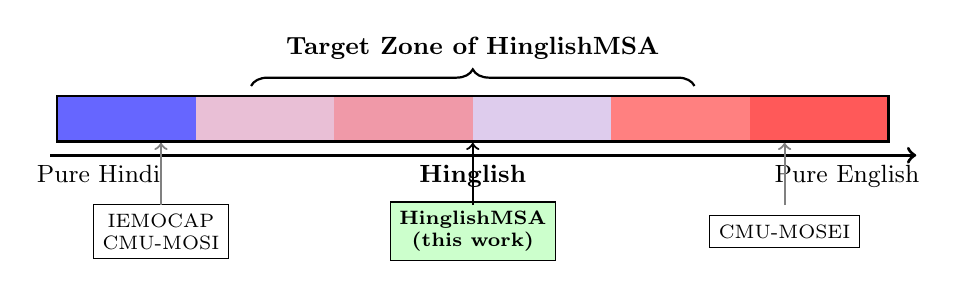
\begin{tikzpicture}[scale=0.88]
% Spectrum bar: discrete color blocks approximating gradient
\fill[blue!60]  (0,0.2)   rectangle (2,0.85);
\fill[blue!35!red!25] (2,0.2) rectangle (4,0.85);
\fill[blue!15!red!40] (4,0.2) rectangle (6,0.85);
\fill[red!35!blue!20] (6,0.2) rectangle (8,0.85);
\fill[red!50]  (8,0.2)   rectangle (10,0.85);
\fill[red!65]  (10,0.2)  rectangle (12,0.85);
\draw[thick] (0,0.2) rectangle (12,0.85);
\draw[->, very thick] (-0.1,0.0) -- (12.4,0.0);
\node[font=\small, anchor=north] at (0.6,  0.0) {Pure Hindi};
\node[font=\small\bfseries, anchor=north] at (6.0, 0.0) {Hinglish};
\node[font=\small, anchor=north] at (11.4, 0.0) {Pure English};
\draw[decorate, decoration={brace, amplitude=6pt}, thick]
    (2.8, 1.0) -- (9.2, 1.0) node[midway, above=6pt, font=\small\bfseries] {Target Zone of HinglishMSA};
\node[draw, fill=white, font=\scriptsize, align=center] at (1.5,-1.1) {IEMOCAP\\CMU-MOSI};
\node[draw, fill=green!20, font=\scriptsize\bfseries, align=center] at (6.0,-1.1) {HinglishMSA\\(this work)};
\node[draw, fill=white, font=\scriptsize, align=center] at (10.5,-1.1) {CMU-MOSEI};
\draw[->, gray, thick] (1.5,-0.72) -- (1.5, 0.18);
\draw[->, thick] (6.0,-0.72) -- (6.0, 0.18);
\draw[->, gray, thick] (10.5,-0.72) -- (10.5, 0.18);
\end{tikzpicture}
\caption{The Hindi--English language continuum. Existing MSA benchmarks occupy the monolingual English endpoint; HinglishMSA is designed to address the under-resourced code-mixed centre.}
\label{fig:cm_spectrum}
\end{figure}

Table~\ref{tab:mixing_examples} catalogues the most common structural mixing patterns observed in the HinglishMSA corpus. What is notable is not just the variety of mixing strategies, but the fact that each one requires a different set of linguistic competencies from an NLP system: a model that handles intra-sentential noun insertion may still fail completely on morphological integration, where English verb stems are inflected with Hindi suffixes.

\begin{table}[ht]
\centering
\caption{Structural patterns of Hinglish code-mixing observed in HinglishMSA, with examples and English glosses}
\label{tab:mixing_examples}
\renewcommand{\arraystretch}{1.35}
\begin{tabular}{p{3.2cm} p{5.0cm} p{4.2cm}}
\toprule
\textbf{Pattern} & \textbf{Hinglish Example} & \textbf{English Gloss} \\
\midrule
Intra-sentential (noun) & \textit{Mujhe yeh movie boring lagi} & I found this movie boring \\
Intra-sentential (verb) & \textit{Usko present karna tha} & He had to present it \\
Script mixing & \textit{aaj mera} \textbf{meeting} \textit{tha} & Today I had a meeting \\
Phonological adaptation & \textit{ismart phone use karo} & Use a smartphone \\
Morphological integration & \textit{woh cry karne laga} & He started to cry \\
Discourse marker insertion & \textit{Actually, mujhe nahi pata tha} & Actually, I didn't know \\
\bottomrule
\end{tabular}
\end{table}

From a computational perspective, Hinglish poses challenges that compound on top of one another in non-obvious ways \cite{aguilar2020lince}. Language identification tools trained on clean monolingual data struggle when Devanagari and Latin characters appear side by side in the same token sequence. ASR systems optimised for either Hindi or English routinely produce garbled transcripts when the input switches between the two mid-sentence. And sentiment lexicons, which underpin many simpler SA systems, rarely cover the emotionally loaded mixing expressions that are most sentiment-bearing in Hinglish speech \cite{winata2019code}. Solving Hinglish NLP requires dealing with all three of these challenges simultaneously --- which is precisely why the research community has made so little progress on it so far.

\section{The Digital Landscape: Why Hinglish Matters Now}

The practical stakes of this research are difficult to overstate. India surpassed 800 million internet users in 2024, and the country's online population is growing faster than that of any other major nation. YouTube reports India as one of its largest markets globally, with content in Hindi and regional languages driving the majority of watch time. A significant share of that content --- travel vlogs, product unboxing videos, political commentary, movie reviews --- is delivered in natural spoken Hinglish by creators whose audiences number in the tens of millions \cite{touvron2023llama}.

For brand managers, healthcare providers, and policy researchers who want to understand what these hundreds of millions of people actually think and feel, existing sentiment analysis tools offer almost nothing. Models trained on English text will misread half the utterances. Models trained on formal Hindi will miss the English-influenced vocabulary that carries most of the sentiment weight. The gap is not a minor inconvenience --- it represents a fundamental inability to access the authentic emotional expression of one of the world's largest online communities.

Figure~\ref{fig:ch1pipeline} traces the full data-collection pipeline developed for this thesis. Starting from YouTube's public Data API and ending with a multimodal feature matrix ready for model training, the pipeline illustrates how a resource-constrained research project can --- with the right combination of open-source tools --- produce a corpus that would previously have required years of manual effort and a large annotation budget.

\begin{figure}[ht]
\centering
\begin{tikzpicture}[
    node distance=0.35cm,
    proc/.style={draw, rounded corners=3pt, fill=blue!8, minimum width=5.8cm,
                 minimum height=0.62cm, align=center, font=\small},
    data/.style={draw, rounded corners=3pt, fill=orange!12, minimum width=5.8cm,
                 minimum height=0.52cm, align=center, font=\scriptsize},
    arr/.style={->, thick}
]
\node[proc] (api)  {YouTube Data API v3};
\node[data, below=0.2cm of api]  (d1)   {1{,}179 video IDs collected};
\node[proc, below=0.2cm of d1]   (dl)   {pytubefix Download + Frame Extraction};
\node[data, below=0.2cm of dl]   (d2)   {1{,}174 videos (WAV audio + JPEG frames)};
\node[proc, below=0.2cm of d2]   (seg)  {ffmpeg silencedetect Segmentation};
\node[data, below=0.2cm of seg]  (d3)   {50{,}695 candidate audio clips};
\node[proc, below=0.2cm of d3]   (face) {OpenCV Haar Cascade Face Detection};
\node[data, below=0.2cm of face] (d4)   {43{,}146 face-confirmed clips};
\node[proc, below=0.2cm of d4]   (asr)  {faster-whisper large-v3 Transcription};
\node[data, below=0.2cm of asr]  (d5)   {29{,}500 transcribed clips};
\node[proc, below=0.2cm of d5]   (hd)   {Hinglish Detection Algorithm};
\node[data, below=0.2cm of hd]   (d6)   {6{,}740 Hinglish clips identified};
\node[proc, below=0.2cm of d6]   (ann)  {Groq llama-3.1-8b-instant Annotation};
\node[data, below=0.2cm of ann]  (d7)   {2{,}652 annotated clips (usable)};
\node[proc, below=0.2cm of d7]   (feat) {MuRIL + wav2vec2-XLSR + CLIP Features};
\node[data, below=0.2cm of feat] (d8)   {\textbf{HinglishMSA Dataset}};

\foreach \a/\b in {api/d1,d1/dl,dl/d2,d2/seg,seg/d3,d3/face,face/d4,
                   d4/asr,asr/d5,d5/hd,hd/d6,d6/ann,ann/d7,d7/feat,feat/d8}
    \draw[arr] (\a)--(\b);
\end{tikzpicture}
\caption{End-to-end HinglishMSA construction pipeline. Each processing stage is shown alongside the number of data items surviving that stage, revealing how the original 50{,}695 candidate clips are progressively refined to the 2{,}652 high-quality annotated clips used for model training.}
\label{fig:ch1pipeline}
\end{figure}

What Figure~\ref{fig:ch1pipeline} also makes visible is the sheer rate of attrition in real-world data collection. Fewer than 6\% of the original candidate clips survive all the way to the final annotated dataset. Every filtering stage --- face detection, Hinglish identification, minimum-confidence annotation --- discards content that would have added noise rather than signal. This aggressive filtering is one of the deliberate design choices of HinglishMSA, and its implications are discussed at length in Chapter~3.

\section{Problem Statement}

Despite the rapid progress in both multimodal sentiment analysis \cite{guo2023recent} and code-mixed NLP \cite{srinivasan2020code}, a critical resource gap persists at their intersection. Three inter-related problems define the challenge this thesis addresses.

\textbf{Problem~1 --- No multimodal Hinglish data exists.} Every established MSA benchmark is recorded in English and annotated by English-speaking workers. No multimodal sentiment dataset has ever been created for Hinglish, or for any code-mixed Indian language. Table~\ref{tab:dataset_comparison} places this gap in quantitative context. The absence of such a resource makes it impossible to train or rigorously evaluate models for this population.

\begin{table}[ht]
\centering
\caption{Comparison of HinglishMSA with established multimodal sentiment benchmarks}
\label{tab:dataset_comparison}
\renewcommand{\arraystretch}{1.3}
\begin{tabular}{lccccc}
\toprule
\textbf{Dataset} & \textbf{Language} & \textbf{Clips} & \textbf{Modalities} & \textbf{Annotation} & \textbf{Year} \\
\midrule
CMU-MOSI \cite{zadeh2016mosi}        & English  & 2{,}199  & T+A+V & Manual crowd       & 2016 \\
CMU-MOSEI \cite{zadeh2018multimodal} & English  & 22{,}856 & T+A+V & Manual crowd       & 2018 \\
IEMOCAP \cite{busso2008iemocap}      & English  & 10{,}039 & T+A+V & Manual (actors)    & 2008 \\
MultiBench \cite{liang2021multibench} & English & varied   & multi & Mixed              & 2021 \\
\midrule
\textbf{HinglishMSA (ours)} & \textbf{Hinglish} & \textbf{2{,}652} & \textbf{T+A+V} & \textbf{LLM-assisted} & \textbf{2026} \\
\bottomrule
\end{tabular}
\end{table}

\textbf{Problem~2 --- English-centric models do not transfer to Hinglish.} Standard BERT \cite{devlin2019bert} and English wav2vec2 \cite{baevski2020wav2vec} fail to adequately represent Hinglish semantics. Hinglish text is cross-script, morphologically mixed, and peppered with transliterated forms that English subword tokenisers either split incorrectly or map to \texttt{[UNK]}. Addressing this requires multilingual pre-training that spans both Hindi and English, as provided by MuRIL \cite{khanuja2021muril} and wav2vec2-XLSR \cite{conneau2021xlsr} --- but no prior work has combined these encoders in a unified multimodal fusion framework specifically designed for Hinglish.

\textbf{Problem~3 --- Manual annotation at scale is not feasible.} Expert bilingual annotation of video clips is expensive and slow. Prior code-mixed sentiment work has necessarily operated on small datasets \cite{joshi2016towards, barman2014code}, which limits statistical power and generalisability. Scalable alternatives --- such as LLM-assisted annotation with confidence filtering --- have not previously been applied to multimodal Hinglish data.

\section{Research Questions}

The work presented in this thesis is organised around five focused research questions that together span the dataset construction, model design, and experimental validation stages of the project:

\begin{description}
    \item[\textbf{RQ1.}] \textit{Can a scalable, LLM-based annotation pipeline produce sentiment labels for Hinglish video content that are reliable enough to train a meaningful downstream model?}

    \item[\textbf{RQ2.}] \textit{Do multilingual pre-trained encoders (MuRIL, wav2vec2-XLSR, CLIP) yield richer feature representations for Hinglish than their English-only counterparts, and does this difference manifest in measurably better sentiment prediction?}

    \item[\textbf{RQ3.}] \textit{Does multimodal fusion --- combining text, audio, and visual modalities --- produce meaningfully better predictions on Hinglish content than any single modality in isolation?}

    \item[\textbf{RQ4.}] \textit{What is the relative contribution of each individual modality to the overall performance of the multimodal model, and are all three modalities necessary?}

    \item[\textbf{RQ5.}] \textit{Does filtering the training corpus by annotation confidence score improve model generalisation, or does the resulting reduction in training data hurt performance more than the noise reduction helps it?}
\end{description}

These questions are addressed empirically in Chapter~4 through a controlled set of ablation experiments. The answers, taken together, constitute the empirical core of this thesis.

\section{Objectives}

The specific research objectives of this thesis are:

\begin{enumerate}
    \item To construct \textbf{HinglishMSA} --- the first multimodal sentiment analysis dataset for code-mixed Hindi-English speech --- comprising 2{,}652 video clips sourced from YouTube, each annotated with a continuous sentiment score in $[-3,+3]$, a text transcription produced by faster-whisper \cite{radford2023whisper}, a raw 16\,kHz WAV audio file, and five JPEG key frames.

    \item To develop an \textbf{improved Hinglish detection algorithm} operating on ASR transcripts, combining Devanagari Unicode co-occurrence statistics, English loanword pattern matching, and dual-language posterior probability estimation. The goal is to reliably separate code-mixed Hinglish clips from monolingual Hindi or monolingual English clips in a large, noisy crawl.

    \item To design and validate an \textbf{LLM-based annotation pipeline} using the Groq inference API and llama-3.1-8b-instant, capable of assigning calibrated continuous sentiment scores to thousands of clips automatically, with a confidence stratification scheme based on score magnitude.

    \item To design and implement \textbf{MulTHinglish} --- a cross-lingual multimodal transformer that integrates MuRIL text representations \cite{khanuja2021muril}, wav2vec2-XLSR audio representations \cite{conneau2021xlsr}, and CLIP visual representations \cite{radford2021clip} through directional cross-modal attention \cite{tsai2019multimodal}, building on the theoretical foundations of the Transformer architecture \cite{vaswani2017attention}.

    \item To conduct a systematic series of \textbf{ablation experiments} that independently vary the active set of modalities and the confidence filtering threshold, quantifying the contribution of each design choice to final model performance.

    \item To establish \textbf{reproducible baselines} on HinglishMSA by releasing the dataset, pre-extracted feature files, and model code publicly, so that future researchers can use HinglishMSA as a standard benchmark for Hinglish affective computing.
\end{enumerate}

\section{Contributions}

This thesis makes five principal contributions:

\begin{enumerate}
    \item \textbf{HinglishMSA Dataset.} A novel multimodal sentiment corpus comprising 2{,}652 video clips drawn from 1{,}174 YouTube videos. Each clip is annotated with a continuous sentiment score in $[-3,+3]$, a faster-whisper transcript, a 16\,kHz audio waveform, and five key frames. At 2{,}652 clips, HinglishMSA is comparable in size to CMU-MOSI \cite{zadeh2016mosi} and is the first multimodal sentiment resource for any code-mixed Indian language variety. The full dataset and feature files are publicly released to support reproducibility and future benchmarking.

    \item \textbf{Three-Stage Hinglish Detection Algorithm.} An automatic method for identifying Hinglish clips in large ASR-transcribed corpora, combining (i) Devanagari Unicode block detection, (ii) English loanword matching in Devanagari context, and (iii) dual-language posterior probability estimation. The algorithm identifies 6{,}740 Hinglish clips from 29{,}500 transcripts, achieving a $6.6\times$ improvement in Hinglish recall relative to a naive single-language baseline (22.8\% vs.\ 3.5\%).

    \item \textbf{Scalable LLM Annotation Pipeline.} An end-to-end annotation system built on the Groq inference API with llama-3.1-8b-instant \cite{touvron2023llama}. The pipeline annotates 2{,}652 clips in approximately two hours, assigns confidence scores based on score magnitude, and supports downstream filtering by confidence level. This demonstrates that LLM-assisted annotation is a practical, low-cost alternative to crowdsourced human annotation for under-resourced, code-mixed languages.

    \item \textbf{MulTHinglish Architecture.} A 5.28-million-parameter cross-lingual multimodal transformer extending MulT \cite{tsai2019multimodal} with multilingual encoders. MulTHinglish achieves a binary sentiment classification accuracy of 70.0\% and an F1-score of 0.702 on HinglishMSA. The best multimodal configuration outperforms a text-only baseline by 28.7 percentage points in binary accuracy, quantitatively demonstrating the value of audio and visual modalities for this task \cite{guo2023recent, poria2017review}.

    \item \textbf{Ablation and Modality Importance Evidence.} Five controlled experimental configurations systematically vary the active modality set and confidence threshold. The results show that all three modalities contribute positively, that their benefits are not additive in isolation, and that cross-modal attention is capturing genuine inter-modality dependencies rather than simply concatenating features. These findings establish empirical baselines that the research community can build on \cite{liang2021multibench}.
\end{enumerate}

\section{Scope and Limitations}

This thesis focuses specifically on \textit{sentiment intensity} as a single continuous dimension, ranging from strongly negative ($-3$) to strongly positive ($+3$). Finer-grained analyses --- multi-class emotion recognition, aspect-level sentiment, sarcasm detection, or stance classification --- are beyond the scope of this work but represent natural next steps \cite{poria2016convolutional, mardjo2022hyvadrf}.

The HinglishMSA corpus is sourced exclusively from YouTube, which introduces a selection bias: YouTube creators tend to be younger, urban, and at least partially English-educated. The corpus therefore may not fully represent the range of Hinglish spoken across India's diverse socioeconomic and geographic landscape. Sentiment annotation is performed by a single LLM rather than a panel of human raters, which introduces the possibility of systematic biases present in the model's pre-training data \cite{touvron2023llama}.

Finally, although MulTHinglish is designed to generalise across Hinglish content, it is evaluated solely on the HinglishMSA test partition. Cross-dataset generalisation to future Hinglish benchmarks remains an open question. The public release of the dataset is intended precisely to enable such evaluations.

\section{Thesis Organisation}

The remainder of this thesis is structured as follows:

\begin{itemize}
    \item \textbf{Chapter~2} surveys the existing literature across four thematic areas: (i) text-based sentiment analysis and its evolution, (ii) multimodal sentiment analysis benchmarks and fusion architectures, (iii) code-mixed NLP with a focus on Hindi-English code-switching, and (iv) cross-lingual pre-trained models. The chapter closes by identifying the specific research gap that motivates this work.

    \item \textbf{Chapter~3} describes the complete system methodology in three parts: the HinglishMSA dataset construction pipeline (from YouTube API query through to LLM annotation); the modality-specific feature extraction procedure for text, audio, and visual streams; and the design, implementation, and training protocol for the MulTHinglish architecture.

    \item \textbf{Chapter~4} presents experimental results across five ablation configurations, analyses the role of each modality, compares performance against CMU-MOSI baselines adapted to the binary task, discusses key findings, and outlines directions for future research.

    \item \textbf{Appendix} provides supplementary material including MulTHinglish hyperparameters, pre-trained model specifications, dataset construction timeline, and feature file inventory.
\end{itemize}

\newpage